\documentclass{article}

\usepackage{graphicx} % Required for inserting images
\usepackage[T1]{fontenc}
\usepackage[utf8]{inputenc}
\usepackage[polish]{babel}

\title{Dokumentacja Projektu Bazy danych 2 \\ \large Inwentaryzacja Sprzętu SKN MOS }

\author{Jakub Maciocha nr. albumu 272949 \and Kornel Uriasz nr. albumu 272967 \and Maciej Pacholczyk nr. albumu 272873}
\date{Październik 2024}

\begin{document}

\maketitle

\newpage
\section{Opis świata rzeczywistego}

    \subsection{Kontekst bieżący}
    Studenckie koło naukowego Microsystem Oriented Society (SKN MOS) prowadzi inwentaryzacje oraz możliwość wypożyczania sprzętu oraz narzędzi dla członków grupy w ramach działania koła naukowego. Siedziba koła zlokalizowana jest w podpiwniczeniu akademika T4 "Czworak", gdzie magazynowany jest sprzęt. Działanie opiera się na rejestrowaniu oraz monitorowaniu sprzętu oraz narzędzi przez administratorów koła naukowego. W tym przypadku są to członkowie zarządu. Katalogują oraz przechowując wszystkie informacje, które są im niezbędne do poprawnego działania koła oraz działania w ramach instytucji Politechniki Wrocławskiej. Taki system w bieżącym momencie pozwala w łatwy sposób zarządzać dostępnymi zasobami.

    \subsection{Opis zasobów ludzkich oraz procesów}
    Proces inwentaryzacji, na moment definiowania nowego systemu, opiera się na fizycznym odnotowywaniu nowego sprzętu z wykorzystanie numerów id lub jego nazwy. Archiwizacja urządzeń odbywa się w formie papierowej, na papierowym arkuszu. Spis sprzętów wypożyczonych prowadzony jest w oddzielnych zasobach w postaci listy  wypożyczeń. Lista ta jest przechowywana również na arkuszu papieru. Proces inwentaryzacji musi być jawny dla klienta jak i dla administratora tj. Klient musi wiedzieć co wypożyczyl i do kiedy musi oddać, administrator musi mieć jawną listę kto co ma, i kiedy ma oddać. Nie może nastąpić sytuacja, kiedy administrator nie wie gdzie jest dany przemiot, jak i nie może wystapić sytuacja, kiedy klient nie wie co ma wypożyczone i do kiedy ma to oddać.
    
    Inwentaryzacja w bieżącym momencie jest prosta, intuicyjna oraz łatwa do przyswojenia dla nowych członków koła, którzy systematycznie dołączają. Proces jest jednak mało wydajny przy zwiększającej się liczbie sprzętu oraz członków koła naukowego. Wzrost ilości dokumentacji dot. sprzętu oraz jego wypożyczeń skutkuje brakiem przejrzystości, trudnościami w archiwizacji oraz lokalizacją sprzętu. Podsumowując proces jest czasochłonny oraz podatny na błędy systemowe.

    W bieżącym momencie osoby działające w obrębie sytemu można podzielić na dwie grupy użytkowników. Pierwsza grupa to użytkownicy z uprawnieniami do odczytu. Klasyfikują się do niej członkowie koła, którzy mogą w swobodny sposób korzystać oraz wypożyczać sprzęt z placówki koła naukowego. W tym momencie do przedstawianego zbioru należy około \textbf{30} członków koła. Druga grupa użytkowników to administratorzy dbający o archiwizację oraz posiadający uprawnienia do wypożyczania sprzętu. Osoby
    te monitorują dostępne zasoby w kole naukowym oraz dbają o przechowywanie dokumentów potwierdzających stan odpowiednich przedmiotów. Do wymienionej grupy należy od \textbf{5 do 10} członków zarządu, którzy stają się administratorami. \newline
    Liczba administratorow : \textbf{5 - 10} \newline
    Liczba klientow : \textbf{30}
    
    Obciążenie serwera jest maksymalnie 10 zapytań na minute, w najgorszym przypadku, w najlepszym jest to 1 zapytanie na godzine.
    \newpage
    \subsection{Wymagania funkcjonalne i niefunkcjonalne}
    Klient (administratorzy) przedstawili następne funkcjonalności dla systemu usprawniającego proces inwentaryzacji oraz wypożyczeń.
        \begin{enumerate}
            \item Funkcjonalne
            
            \begin{enumerate}
                \item Aplikacja przedluża okres wypożyczenia na życzenie klienta, po zatwierdzeniu przez administratora
                \item Aplikacja ponagla o oddanie przedmiotu na zapytanie administratora
                \item Aplikacja decyduje o prawidłowym/nieprawidłowym oddaniu przedmiotu na podstawie daty wypożyczenia oraz aktualnej daty
                \item Aplikacja pokazuje przefiltrowane dane na żądanie klienta
                \item Aplikacja weryfikuje uprawnienia klienta
                \item Aplikacja wysyła powiadomienia o upływającym terminie wypożyczeń
                \item Aplikacja generuje miesięczne raporty sprzętowe
            \end{enumerate}

            \item Niefunkcjonalne 

            \begin{enumerate}
                \item Lokalizacja serwera w pokoju socjalnym w siedzibie koła naukowego
                \item Strona posiada przejrzysty interfejs
                \item Strona jest atrakcyjna/estetyczna
                \item Aplikacja jest umieszczona na serwerze koła naukowego
                \item Aplikacja przestrzega obostrzeń RODO
            \end{enumerate}
            
        \end{enumerate}

Diagram przypadkow uzycnia

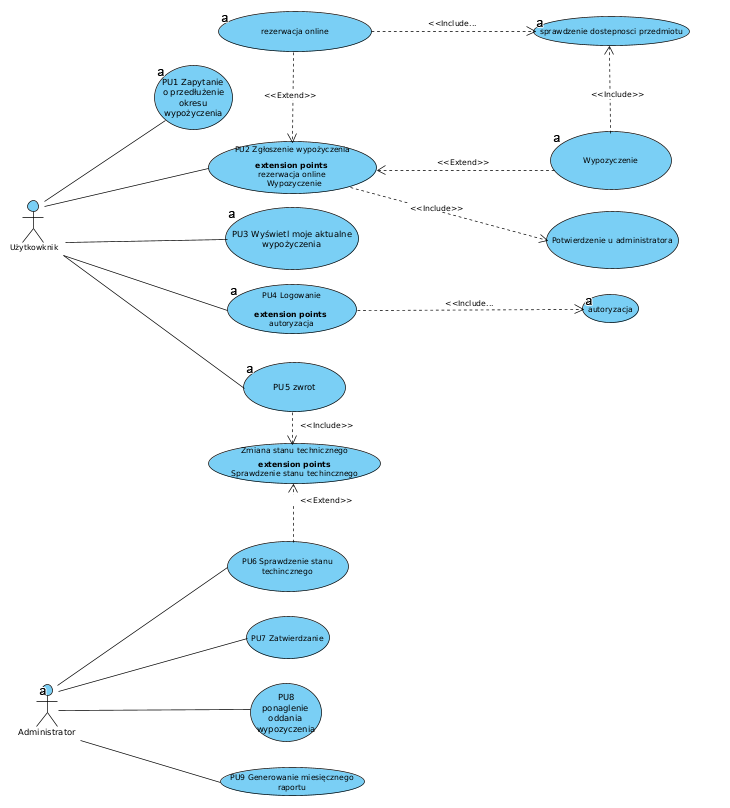
\includegraphics[width=\textwidth]{media/use_case.png}

\end{document}
